\subsection{Opacity Due to Bound-Free Absorption}
Bound-free \h\ is the dominant contribution to opacity in the solar atmosphere for photons in the infrared (with wavelength $\lambda \gtrsim 1.6 \mu$m), optical, and ultraviolet regimes; since the solar luminosity peaks in this wavelength range \h\ opacity affects a significant portion of the light coming from the sun.

\cite{wishart1979} calculates the bound-free photoionization
cross-section of \h\ using close-coupling plus correlation
wavefunctions as a function of photon
over the wavelength range 1250-16300 $\AA$.  The cross-sections given
in that reference are accurate to within 1\%.
The calculated cross sections are shown as the points in
figure~\ref{fig:bfcrosssection}; the lines connecting the points are a
cubic spline interpolation.  The right side of the figure shows the
cross-section for photons with energies close to the $0.75$ eV
sufficient to ``ionize'' the \h ion to become H.  The cross-section
peaks at $\sim 8500$\AA and then decreases with increasing photon
energy.  It is interesting to note that this cross-section peaks in
the optical with large values in the near infrared and near
ultraviolet, just as does solar spectrum.  Hence, the \h\ opacity is
most relevant is the regime of photon energies where the sun's own
photon production peaks.  This coincidence causes the \h\ opacity to
be even more dominant in the sun than in stars with a similar \h\
density in their atmospheres but with a photon energy spectrum peaking
outside the optical.
\begin{figure*}{h}
\includegraphics[width=150mm]{figs/boundfree_crosssection.pdf}
\caption{\label{fig:bfcrosssection}The bound-free photoionization
cross-section of \h. Tabulated values calculated
by \cite{wishart1979} are given as open circles with a cubic spline
interpolation shown as the line connecting the points.  The calculated
cross-sections span from near infrared (at the wavelengths where photon
energies are sufficiently high to ionize the least bound electron
of \h) to near ultraviolet. As shown, photon energy increases along
the x-axis from right to left.}
\end{figure*}

Figure~\ref{fig:bohmopacity} shows  opacity as a function of wavelength over the range of wavelengths where \h\ bound-free opacities are relevant for a theoretical solar-like star.  At high wavelengths, past the $\sim 1.6 \mu$m cutoff for \h\ opacity free-free interactions with \h\ dominate the opacity (the H in the figure is a typo, it should be \h), while at lower wavelengths Balmer bound-free absorption begins to dominate the opacity.
\begin{figure}{h}
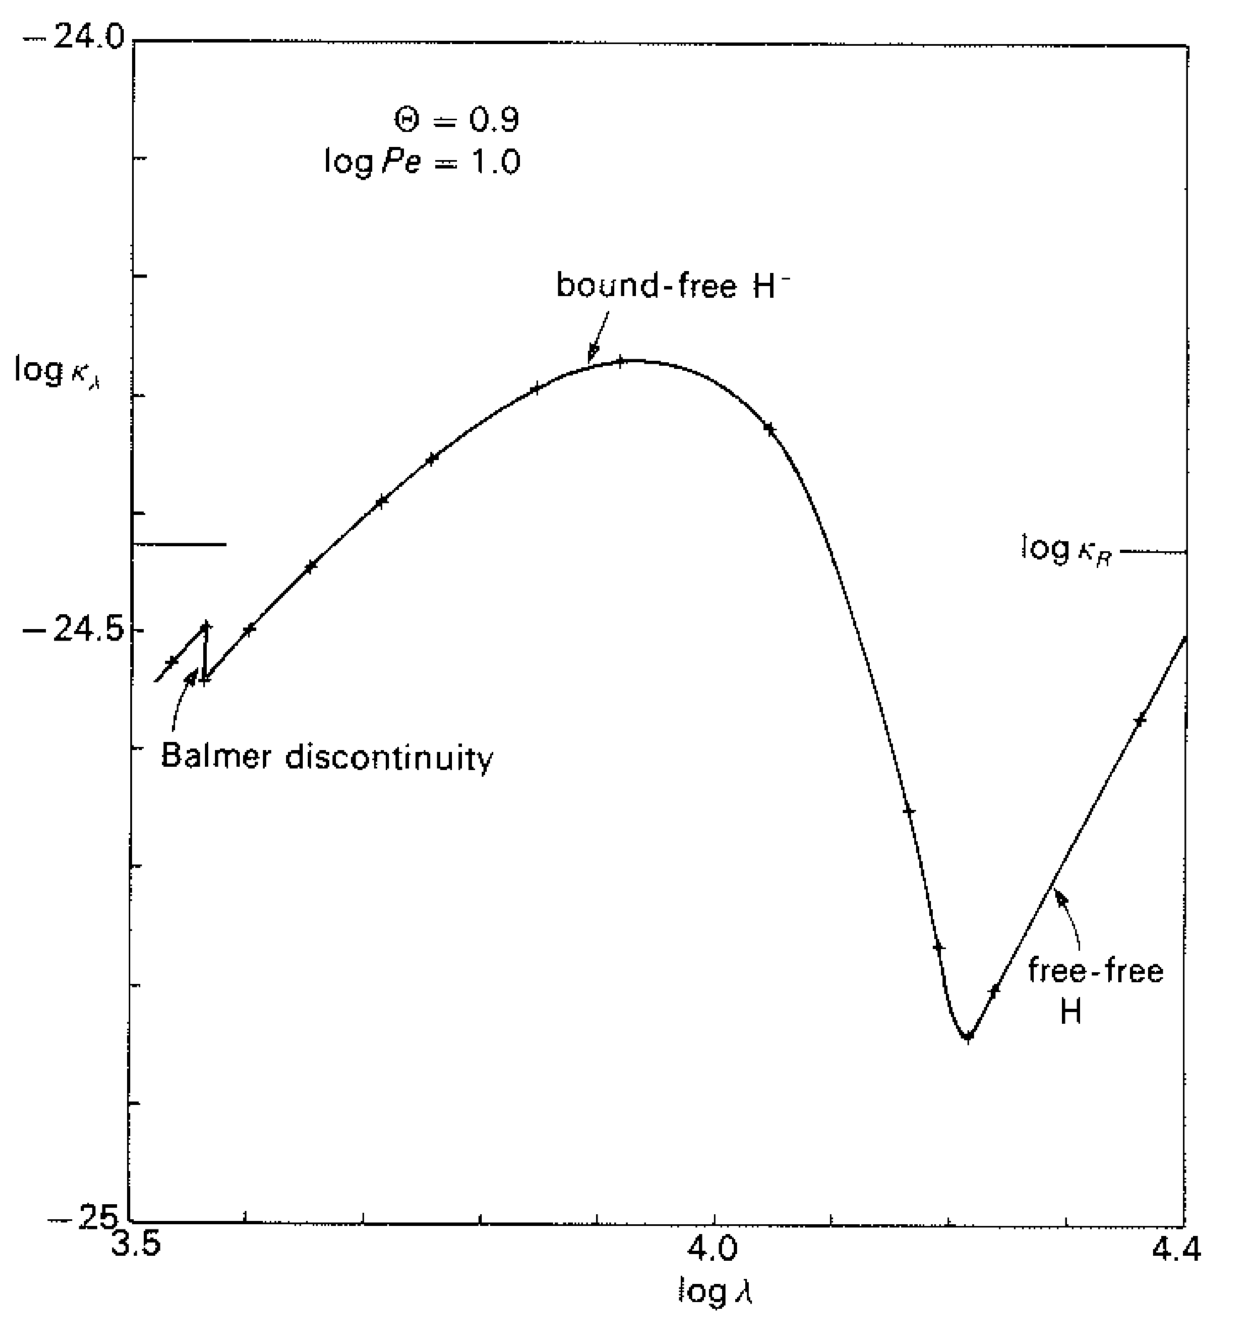
\includegraphics[width=80mm]{figs/hminusopacity.png}
\caption{\label{fig:bohmopacity}Continuous absorption coefficient per heavy particle, shown for $\Theta=0.9$ (which means $T=5600$ K and log $P_e=1.0$.  Note that the free-free contribution is mislabelled; it should be free-free from \h\ not H.  Figure from \cite{boehm1989}.}
\end{figure}

Figures~\ref{fig:bfcrosssection} and \ref{fig:bohmopacity} both show that the opacity doesn't show a discontinuity at the $\sim$1.6$\mu$m cutoff value for \h\ ``ionization'' as would be expected and is indeed seen for other species being ionized.  Figure~\ref{fig:bethe} (taken from \citealt{bethe1977}) shows $\sigma$ as a function of photon frequency relative to the frequency corresponding to the ionization energy $\nu$ for H, He, and \h.  H and He both show a large cross-section right at the threshold frequency which decays with increasing frequency; \h, however, shows a small cross-section right at the threshold which increases and reaches a maximum at $\nu/\nu{thr}\sim$1.7.  \cite{rau1996} explains this in terms of basic quantum mechanics and angular momentum.  After a photon is absorbed by \h\ the electron departs in a $p$-wave.  In the ground state of \h, however, both the electrons are in the $s$ orbital.  Thus there is an angular momentum barrier that must be overcome, via quantum tunnelling.  Just above the ionization threshold electrons have low energy and see the angular momentum barrier as the longest range potential; the probabilities associated with tunnelling through this barrier thus affect the cross-section at these low energies. .  {\bf Can talk about Wigner 1948 E to the l+1/2 if you want. Rau page 116}.  This is not the case for neutral atoms, where the Coulomb potential is the longest-range potential.  This potential has no dependence on angular momentum and, as such, there is no angular dependence on the cross-section.
\begin{figure}{h}
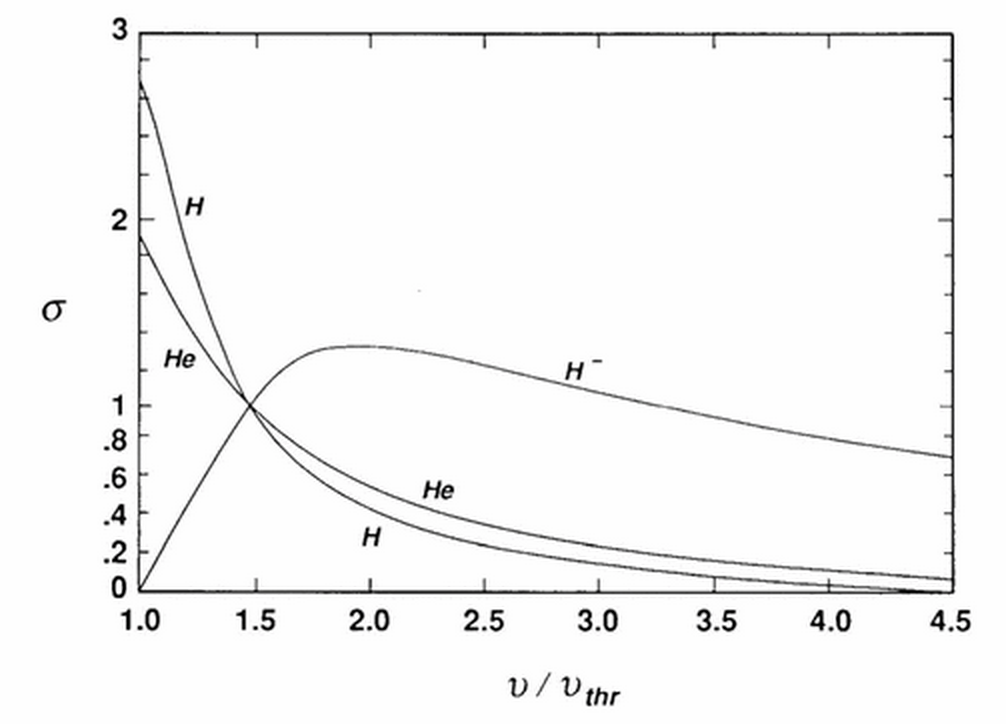
\includegraphics[width=80mm]{figs/betheplot.png}
\caption{\label{fig:bethe}Photoionization cross-section as a function of photon frequency, expressed in the unitless ratio $\nu/\nu_{thr}$, which is the ratio of the photon frequency relative to frequency of a photon with energy corresponding to the ionization energy of the species.  Cross-sectionsH, He, and \h\ are shown (from \citealt{bethe1977}).}
\end{figure}

\subsection{Opacity Due to Bound-Free Absorption}
At wavelengths greater than $\sim1.6\nu$m free-free absorption on \h\ provides a significant contribution to the opacity.  Free-free absorption, also known as inverse Bremstrahlung absorption, is the process by which an electron absorbs a photon in the presence of an electric field provided by an atom or ion.  For \h\ the process looks like
\beq
\gamma + e^- + H^- \rightarrow e^- + H^-.
\eeq
\cite{bell1987} calculate the absorption coefficient for free-free absorption on \h\ for various temperatures.  They include s $\leftrightarrow$ p and p $\leftrightarrow$ d transition contributions only, saying that contributions from higher partial waves are negligible.  They use the notation $\theta=5040 K /T$. Their calculations are shown in table~\ref{tab:freefreetable}.  It is worth noting that the free-free absorption coefficient increases with increasing wavelength, allowing it to contribute significantly to the opacity at wavelengths longer than the $\sim 1.6\nu$m cutoff for \h\ bound-free absorption.  The absorption coefficient also increases with decreasing temperature (represented by increasing $\theta$).  For reference purposes,  the sun has $\theta=0.87$.
\begin{table}
\caption{\label{tab:freefreetable}\h\ free-free absorption coefficient as calculated by \cite{bell1987}}
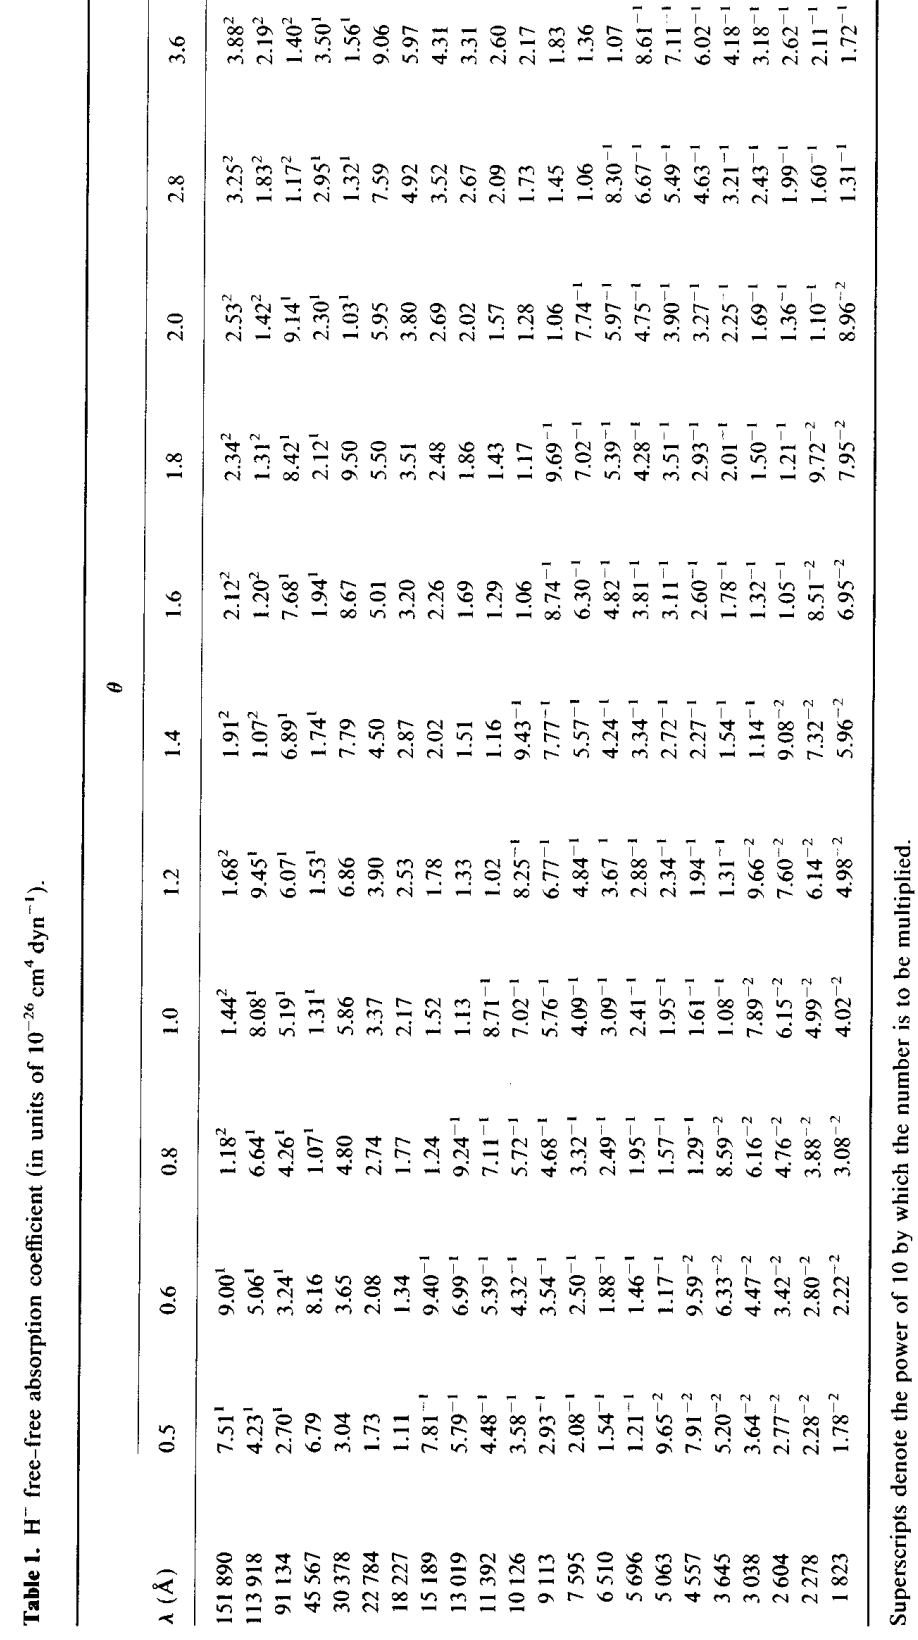
\includegraphics[width=\linewidth]{figs/freefreetable.png}
\end{table}

This brings up the question about how the absorption coefficient contribution from \h\ changes at $\sim 1.6 \mu$m, where bound-free absorption becomes relevant.  Table~\ref{tab:boundfreecomp}, taken from \cite{bell1975} provides a partial answer.  Please note in table~\ref{tab:boundfreecomp} that the top line beginning with $\lambda$ should read ``$\lambda(\AA)\theta=$''. The $\theta$ is not clear in the grainy rendition of the table.  This is the same $\theta$ as in table~\ref{tab:freefreetable}.  Moving from 18225 \AA\ to 15188 \AA, over the wavelength range where bound-free absorption starts to become relevant, the coefficient for $\theta=$0.8 decreases\footnote{Although the exact nature of the decrease for $\theta=$0.8 is hidden in the low wavelength resolution of the table, over the range of $\sim$300 \AA between 18225 \AA\ to 15188 \AA\ the coefficient may reach a minimum and start to increase again and still produce the numbers we see in table~\ref{tab:boundfreecomp}.} while for the other $\theta$ it increases, although in some cases only modestly. Larger $\theta$, corresponding to lower temperature, produce a larger increase in the absorption coefficient in this range.  The modest increase at higher temperatures may seem puzzling at first but a quick review of figure~\ref{fig:bethe} reminds us that the bound-free absorption cross-section for \h\ does not exhibit a sudden jump at the cutoff wavelength as would be seen for other species undergoing photoionization, but rather increases fairly modestly, reaching a maximum only for wavelengths less than the cutoff wavelength.  For the next tabulated value of wavelength, $\lambda=11391$\AA, all absorption coefficients are shown to be increasing.  This table reflects the somewhat gradual transition from \h\ free-free absorption to \h\ bound-free absorption as being the dominant contribution of \h\ to the opacity, as can be seen in figure~\ref{fig:bohmopacity}, in contrast with the sudden increase in opacity from Balmer bound-free absorption seen in the same figure.
\begin{table}
\caption{\label{tab:boundfreecomp}\h\ total absorption coefficient as calculated by \cite{bell1975}}
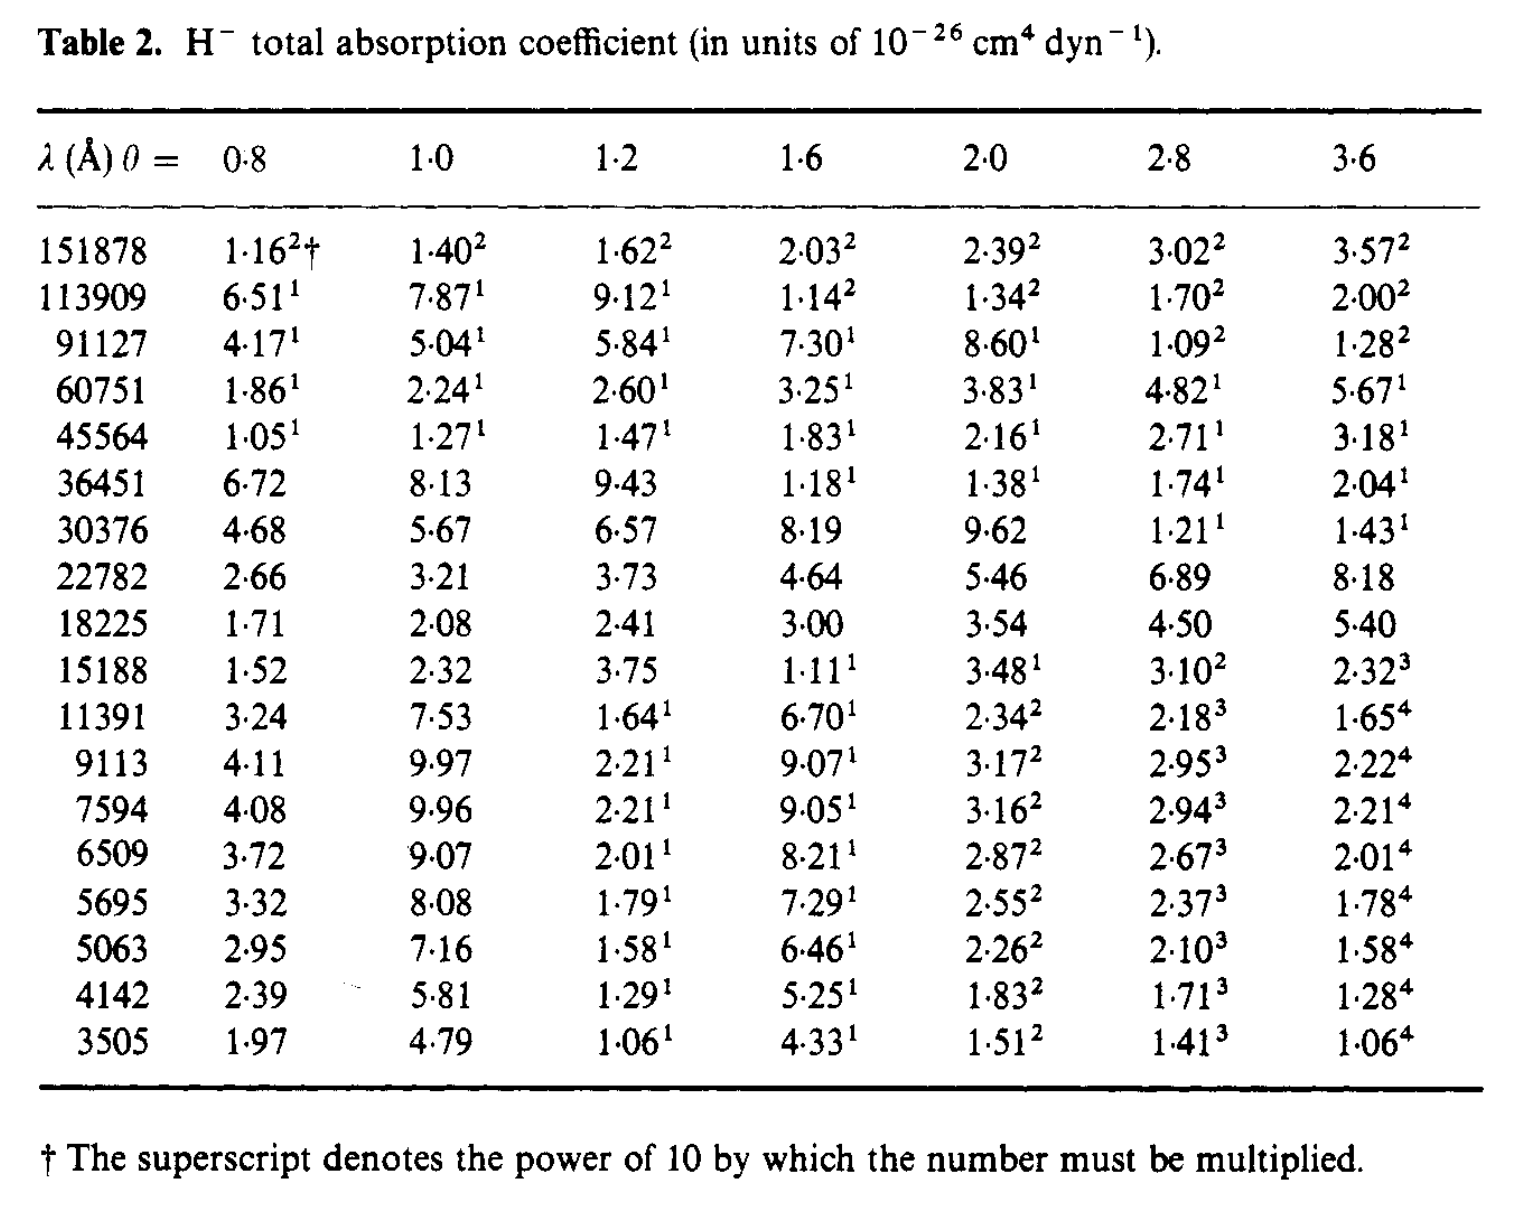
\includegraphics[width=\linewidth]{figs/freeandboundtable.png}
\end{table}

It would be nice to compare directly the values of table~\ref{tab:freefreetable} with those used to generate figure~\ref{fig:bfcrosssection} but they are in different units so direct comparison is not possible as is.  However, \cite{chandra1946} provide an early theoretical calculation of the total absorption coefficient due to both free-free and bound-free absorptions for \h, shown in figure~\ref{fig:chandratotal}.  In this figure the total absorption coefficient has a local minimum around $\sim1.65\mu$m, close to the cutoff wavelength for \h\ bound-free absorption (at $T$=6300 K).  Thus, although the bound-free contribution is smaller than the free-free contribution around the cutoff wavelength, it immediately begins to have a significant effect on the total absorption coefficient, at $T$=6300 K at least.  Figure~\ref{fig:bohmopacity} shows a minimum somewhere between $\sim$14000-16000\AA\ for her calculation of the opacity at $T$=5600 K and $P_e=1.0$.  She also makes the comment that the sum of the free-free and bound-free contributions to the opacity has a minimum between $\sim$16000-16500\AA. Thus it appears that, in the sun, the bound-free contribution to the absorption coefficient becomes significant either right at or within a few hundred \AA ngstrom of the cutoff wavelength.
\begin{figure}
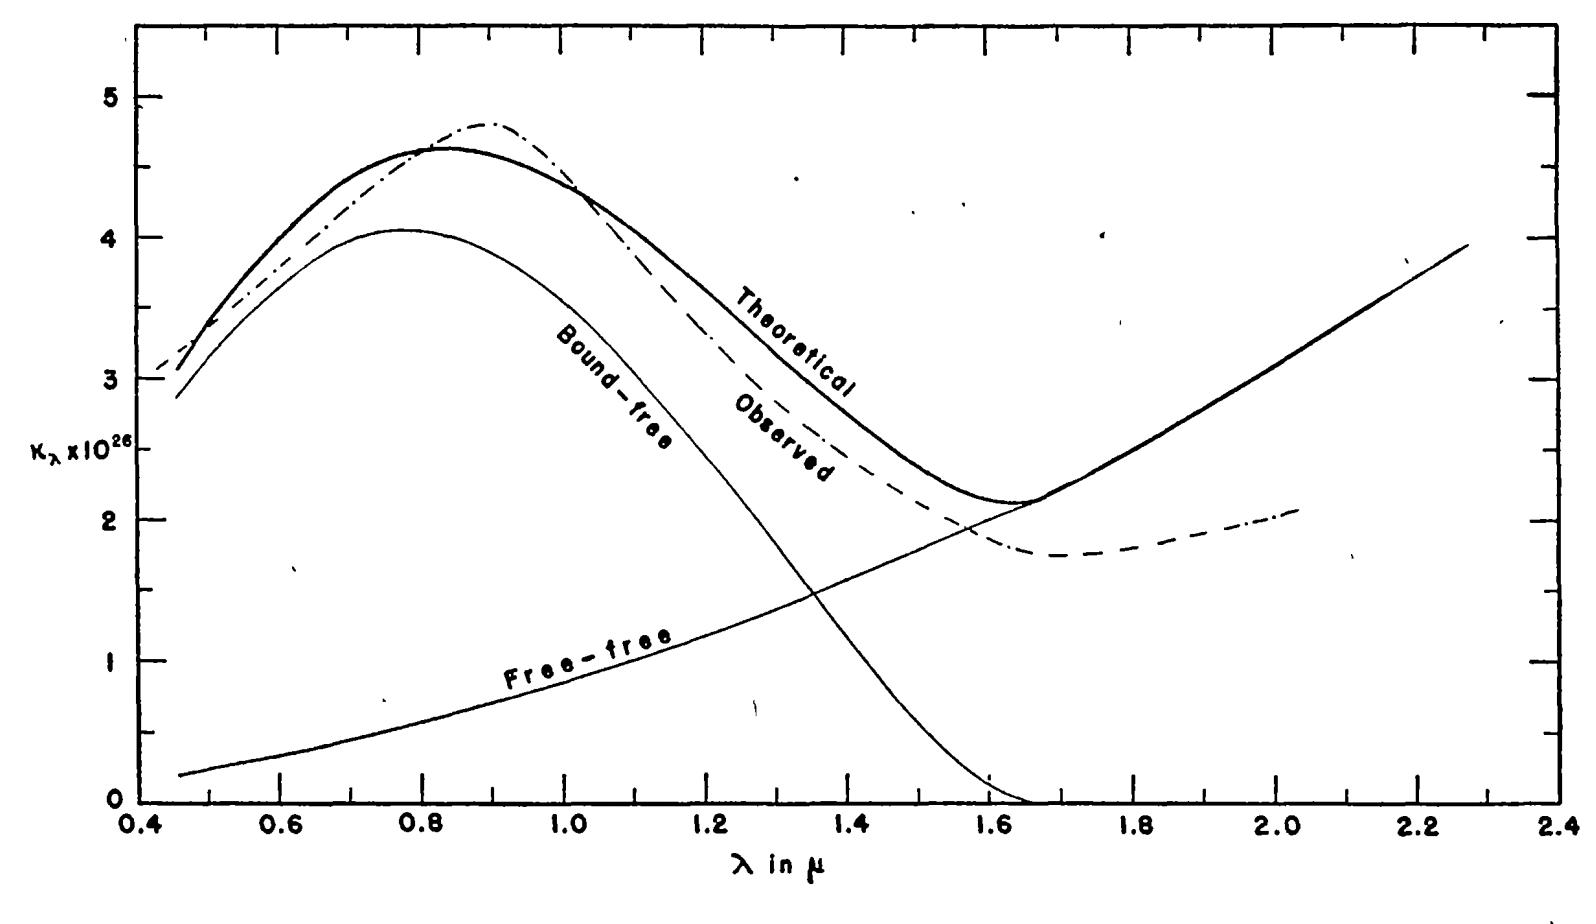
\includegraphics[width=\linewidth]{figs/chandraopacity.png}
\caption{\label{fig:chandratotal}From \cite{chandra1946}, the continuous absorption coefficient of \h\ per neutral hydrogen atom per unit electron pressure for a temperature of 6300 K.  A comparison with the observed values is made, shown with the dotted line.  The curve marked ``theoretical'' represents the sum of the free-free and bound-free curves.}
%M&B and W&W correspond to earlier determinations of the same quantities, by Massey and Bates (bound-free) and  \cite{wheeler1942} (free-free) respectively. No further reference to Massey and Bates other than their names could be found in \cite{chandra1946}.
\end{figure}

Plunk in somewhere: free-free
\begin{equation}
\kappa = \frac{3.7062}{k(k^2+0.05512)}\left\lvert \int_0^{infty}W)x(r)\chi_1(r)dr \right\rvert^2 \times 10^{-18} \textrm{cm}^2
\end{equation}
where $k$ is the momentum of the ejected electron in atomic units, $W_2(r)$ is a certain weight function which can be tabulated (values are shown in \citealt{chandra1945}, and $\chi_1(r)$ is the radial part of a p-spherical wave in the Hartree field of a hydrogen atom which tends ot unit amplitude at infinity (\citealt{chandra1945}).
